%=============================================================================
%\documentclass[11pt,twoside]{article}
\documentclass[11pt,a4paper,twoside,bibtotoc]{scrartcl}
%\documentclass[twoside,11pt]{article}
%\usepackage{jnm}
%=============================================================================
\usepackage{a4wide}
\usepackage{amsfonts}
\usepackage{amsmath}
\usepackage{theorem}
%\usepackage{jkmath}
\usepackage{subfigure}
\usepackage{natbib}
\usepackage{algorithm}
\usepackage{algorithmic}
\usepackage{graphicx}
\usepackage{xcolor}
\usepackage{showkeys}

\theoremstyle{plain}
\newtheorem{theorem}{Theorem}[section]
\newtheorem{corollary}[theorem]{Corollary}
\newtheorem{lemma}[theorem]{Lemma}
\newtheorem{proposition}[theorem]{Proposition}
\theoremstyle{definition}
\newtheorem{definition}[theorem]{Definition}
\newtheorem{example}[theorem]{Example}
\theoremstyle{remark}
\newtheorem{remark}[theorem]{Remark}
\newenvironment{proof}{{\bf Proof.}}{$\Box$}

\newcommand{\adj}{{\vdash \hspace*{-1.72mm} \dashv}}
\newcommand{\supp}{\:{\rm supp}}

\renewcommand{\topfraction}{1}
\renewcommand{\textfraction}{0}
\setcounter{totalnumber}{4}

%============================================================================

\newcommand{\N}{\ensuremath{\mathbb{N}}}
\newcommand{\NZ}{\ensuremath{\mathbb{N}_{0}}}
\newcommand{\Z}{\ensuremath{\mathbb{Z}}}
\newcommand{\Q}{\ensuremath{\mathbb{Q}}}
\newcommand{\R}{\ensuremath{\mathbb{R}}}
\newcommand{\Rp}{\ensuremath{\mathbb{R}^{+}}}
\newcommand{\Rn}{\ensuremath{\mathbb{R}^n}}
\newcommand{\Rnn}{\ensuremath{\mathbb{R}^{n \times n}}}
\newcommand{\C}{\ensuremath{\mathbb{C}}}
\newcommand{\Pol}{\ensuremath{\Pi}}

\newcommand{\norm}[1]{\ensuremath{\left\|#1\right\|}}
\newcommand{\abs}[1]{\ensuremath{\left\vert#1\right\vert}}
\newcommand{\set}[1]{\ensuremath{\left\{#1\right\rbrace}}
\newcommand{\pset}[3]{\ensuremath{\left\{#1\ \left#2\ #3\right.\right\rbrace}}
\newcommand{\veps}{\ensuremath{\varepsilon}}
\newcommand{\vtheta}{\ensuremath{\vartheta}}
\newcommand{\vphi}{\ensuremath{\varphi}}
\newcommand{\towards}{\ensuremath{\longrightarrow}}

\newcommand{\twosphere}{\ensuremath{\mathbb{S}^2}}
\newcommand{\Ln}[2]{\ensuremath{\text{\rm{L}}^{#1}\left(#2\right)}}
\newcommand{\interv}[4]{\ensuremath{\left#1\left.#2,#3\right#4\right.}}
\newcommand{\fun}[2]{\ensuremath{#1{\hspace{-0.4ex}}\left(#2\right)}}
\newcommand{\paren}[1]{\ensuremath{\left(#1\right)}}
\newcommand{\encl}[3]{\ensuremath{\left#1#2\right#3}}
\newcommand{\bigo}[1]{\ensuremath{\mathcal{O}\paren{#1}}}
\newcommand{\smallo}[1]{\ensuremath{\mathcal{o}\paren{#1}}}
\newcommand{\spacer}{\ensuremath{{}^{}}}
\newcommand{\scalarproduct}[2]{\ensuremath{\left<#1,#2\right>}}
\newcommand{\mb}[1]{\mathbf{#1}}
\newcommand{\V}[1]{\mb{#1}}
\newcommand{\transp}{\text{\rm{T}}}
\newcommand{\h}{\text{\rm{H}}}
\newcommand{\dx}{\text{\rm{d}}}
\renewcommand{\Re}{\text{\rm{Re}}}
\renewcommand{\Im}{\text{\rm{Im}}}
\newcommand{\e}{\mbox{\rm{e}}}
\newcommand{\im}{\mbox{\scriptsize\rm{i}}}
\newcommand{\diag}{\text{\rm{diag}}}
\def\invisible#1{\textcolor{white}{#1}}
\newcommand{\ceil}[1]{\encl{\lceil}{#1}{\rceil}}
\newcommand{\floor}[1]{\encl{\lfloor}{#1}{\rfloor}}

%============================================================================

\numberwithin{equation}{section}
\numberwithin{table}{section}
\numberwithin{figure}{section}

%\newlength{\temp}
%\setcounter{totalnumber}{10}
%\setcounter{topnumber}{10}

%============================================================================

\title{
%{\rm\normalsize Short Note}\\
Fast Summation of radial functions on the sphere}

\date{\today}

\author{
Jens Keiner\thanks{keiner@math.uni-luebeck.de, University of
  L\"ubeck, Institute of Mathematics, D--23560 L\"ubeck} \and
Stefan Kunis\thanks{kunis@math.uni-luebeck.de, University of
  L\"ubeck, Institute of Mathematics, D--23560 L\"ubeck} \and
Daniel Potts\thanks{potts@math.uni-luebeck.de, University of
  L\"ubeck, Institute of Mathematics, D--23560 L\"ubeck} 
}

%=============================================================================
\begin{document}
\maketitle

\begin{abstract}
\medskip

%\noindent
%2000 {\it Mathematics Subject Classification}. 65F10, 65F15, 65T40.

\noindent
{\it Radial functions are a powerful tool in many areas of multi-dimensional 
approximation. We present a fast approximative algorithm for the evaluation of
a linear combination of radial functions on the sphere $\mathbb{S}^2$. The 
approach is based on an approximation to the corresponding Gramian matrix
and fast algorithms for the computation of spherical Fourier transforms.}
\end{abstract}


%%%%%%%%%%%%%%%%%%%%%%%%%%%%%%%%%%%%%%%%%%%%%%%%%%%%%%%%%%%%%%%%%%%%%%%%%%%%%%%
\section{Introduction}\label{sect:1}
%%%%%%%%%%%%%%%%%%%%%%%%%%%%%%%%%%%%%%%%%%%%%%%%%%%%%%%%%%%%%%%%%%%%%%%%%%%%%%%

Radial basis functions are a powerful tool in many areas of multi-dimensional 
approximation and interpolation.
In radial basis function methods one approximates functions from $\R^3
\rightarrow \R$ by linear combinations of radial symmetric translates 
$\fun{\Phi}{\V{y} - \cdot \,}$, $\V{y} \in \R^3$, of a single function $\phi : \R^{+} \rightarrow \R$, i.e. 
\[
  \fun{\Phi}{\V{y} - \cdot \,}:\R^3 \rightarrow \R, \, \V{x} \mapsto \phi(\|\V{y} - \V{x}\|_2).
\]
The spherical counterpart are the \emph{zonal functions} which depent solely
on the geodesic distance of two points on the sphere $\twosphere:=\{
\V{\xi} \in \twosphere: \|\V{\xi}\|_2=1\} \subset \R^3$. The norm $\|\V{y} - \V{x}\|_2$ 
is replaced by the usual inner product.

More formally, let $K \in \Ln{2}{\interv{[}{-1}{1}{]}}$ and define for fixed
$\V{\eta} \in \twosphere$ the $\V{\eta}$-zonal function 
\[
  \fun{K}{\V{\eta} \: \cdot \,}: \twosphere \rightarrow \R,\ \V{\xi} \mapsto
  \fun{K}{\V{\eta} \cdot \V{\xi}}\,.% \qquad \V{\xi} \in \twosphere.
\]

The formal description of the problem we will address is as follows:
Given $D,L \in \N$, a set of arbitrary \emph{source nodes} $\mathcal{Y} :=
\{\V{\eta}_{l} \in \twosphere: l = 0,\ldots,L-1\}$, and a vector of
real coefficients $\V{b}:=(b_{l})_{l=0}^{L-1}$, evaluate the sum
\begin{equation}
  \label{Applications:KernelSum}
  \fun{f}{\V{\xi}} := \sum_{l = 0}^{L-1} b_{l} \fun{K}{\V{\eta}_{l} \cdot \V{\xi}}
\end{equation}
on a set of arbitrary \emph{target nodes} $\mathcal{X} := \{\V{\xi}_{d}
  \in \twosphere: d=0,\ldots,D-1\}$.

The naive approach for evaluating \eqref{Applications:KernelSum} leads to
an $\bigo{LD}$ algorithm if we assume that the zonal function
$\fun{K}{\V{\eta} \: \cdot}$ can be evaluated easily or all values
$\fun{K}{\V{\eta}_{l} \cdot \V{\xi}_{d}}$ can be stored in advance. 
For large $L$ and $D$ the computational effort becomes quickly unaffordable.
The \emph{panel clustering method} on the sphere in \cite{FrGlSch98} reduces the
computational effort for evaluating \eqref{Applications:KernelSum} based on the
traditional method of dividing the evaluation into a near- and a far-field:
For every zonal function $\fun{K}{\V{\eta}_l \: \cdot}$, the near-field
contribution is calculated exactly whereas the contribution of the far-field
is approximated coarsely.
We present an approximative algorithm with arithmetic complexity 
${\cal O} (D+L)$ based on the \emph{nonuniform fast spherical Fourier 
transform (NFSFT)}, cf. \cite{kupo02}. 

The remainder of this paper is organized as follows:
To keep the paper self-contained, we summarize definitions and properties
of Fourier expansions of zonal functions in Section 2.
In Section 3, we propose our fast scheme for the evaluation of
\eqref{Applications:KernelSum}, whereas Section 4 establishes
error estimates for a variety of functions $K$.
Finally, Section 5 presents numerical experiments.

%%%%%%%%%%%%%%%%%%%%%%%%%%%%%%%%%%%%%%%%%%%%%%%%%%%%%%%%%%%%%%%%%%%%%%%%%%%%%%%
\section{Prerequisites} \label{sect:2}
%%%%%%%%%%%%%%%%%%%%%%%%%%%%%%%%%%%%%%%%%%%%%%%%%%%%%%%%%%%%%%%%%%%%%%%%%%%%%%%

The \emph{Legendre polynomials} $P_k : \interv{[}{-1}{1}{]} \rightarrow \R$, $k \in
\N_{0}$, as classical orthogonal polynomials are given by their
\emph{Rodrigues formula} 
\[
\fun{P_k}{x} := \frac{1}{2^k k!} \frac{\dx^k}{\dx x^k} \paren{x^2-1}^k.
\]
One verifies
\begin{equation}\label{leg_prop}
\fun{P_{k}}{\pm1} = \paren{\pm1}^{k}, \quad
\max_{x \in \interv{[}{-1}{1}{]}} \abs{\fun{P_{k}}{x}} = 1,\text{ and} \quad
\left|\fun{P_{k}}{\cos\vartheta}\right| \le \sqrt{\frac{2}{\pi k
    \sin\vartheta}},
\end{equation}
where the last inequality holds for $\vartheta \in (0,\pi)$ and $k \ge 1$, see
e.g. \cite[pp. 47]{niuv}.
Furthermore, two recurrence relations are given by
\begin{equation}\label{three1}
\paren{k+1}\fun{P_{k+1}}{x} = \paren{2k+1}x\fun{P_{k}}{x} - k\fun{P_{k-1}}{x}
\end{equation}
and
\begin{equation}\label{three2}
\paren{2k+1} \fun{P_{k}}{x} = \fun{P_{k+1}'}{x} - \fun{P_{k-1}'}{x}.
\end{equation}
The more general \emph{associated Legendre functions} $P_{k}^n$, $k \in \NZ$, $n \le k$, are defined by
\[
  \fun{P_{k}^n}{x} := \left(\frac{(k-n)!}{(k+n)!}\right)^{1/2} 
  \left(1-x^2\right)^{n/2} \frac{\dx^n}{\dx x^n} \fun{P_{k}}{x}.
\]

In spherical coordinates, a point $\V{\xi} \in \twosphere$ is identified with 
a vector $(\vartheta,\varphi) \in [0,\pi] \times [-\pi,\pi)$. 
Let the space of real-valued continuous functions on the sphere be decomposed
into the direct sum of spaces of \emph{spherical harmonics}, i.e.
$C(\twosphere)=\bigoplus_{k=0}^{\infty} \mathcal{H}_k$. We denote by 
$\set{Y_{k}^n}_{k \in \NZ; n=-k,\ldots,k}$ the 
standard $\text{L}^2$-orthonormal basis of spherical harmonics given by
\[
  \fun{Y_{k}^n}{\V{\xi}} = \fun{Y_{k}^n}{\vartheta,\varphi} := 
  \sqrt{\frac{2k+1}{4\pi}} 
  \fun{P_{k}^{|n|}}{\cos\vartheta} \e^{\im n \varphi}.
\]
The orthogonal expansion in terms of the basis functions $Y_k^n$ 
of the zonal function $\fun{K}{\V{\eta} \: \cdot \,}$ is given by
\begin{equation}
  \label{equation:kernelExpansion}
  \fun{K}{\V{\eta} \cdot \V{\xi}} = \sum_{k = 0}^{\infty} \sum_{n=-k}^k
  \fun{K^{\wedge}}{k}\overline{\fun{Y_{k}^n}{\V{\eta}}} \fun{Y_{k}^n}{\V{\xi}}
  = \sum_{k = 0}^{\infty} \frac{2k+1}{4\pi} \fun{K^{\wedge}}{k}
  \fun{P_{k}}{\V{\eta} \cdot \V{\xi}}.
\end{equation}
Here, we use the addition theorem
\[
\sum_{n=-k}^{k} \overline{\fun{Y_{k}^n}{\V{\eta}}} \fun{Y_{k}^n}{\V{\xi}} =
    \frac{2k+1}{4\pi}\fun{P_k}{\V{\eta} \cdot \V{\xi}}
\]
and the \emph{Fourier-Legendre coefficients} $\fun{K^{\wedge}}{k}$ of $K$ are given for $k \in \NZ$
by
\begin{equation}
  \label{equation:legtrafo}
  \fun{K^{\wedge}}{k} := 2 \pi \int_{-1}^{1} \fun{K}{x} \fun{P_{k}}{x} \dx 
  x\,.
\end{equation}

\begin{remark}
Of course, to every radial function $\phi(\|\V{\eta} - \cdot \,\|_2)$ corresponds a zonal function 
$\fun{K}{\V{\eta} \: \cdot \,}$ by means of 
\[
  \fun{K}{\V{\eta} \cdot \V{\xi}} := \phi\left(\sqrt{2-2\V{\eta} \cdot
  \V{\xi}}\right)\,.
\]
The relation between radial basis functions and their corresponding zonal
functions is considered in detail in \cite{CaFi}.
\end{remark}

%%%%%%%%%%%%%%%%%%%%%%%%%%%%%%%%%%%%%%%%%%%%%%%%%%%%%%%%%%%%%%%%%%%%%%%%%%%%%%%
\section{Fast Summation}
%%%%%%%%%%%%%%%%%%%%%%%%%%%%%%%%%%%%%%%%%%%%%%%%%%%%%%%%%%%%%%%%%%%%%%%%%%%%%%%
Basically, the first representation in \eqref{equation:kernelExpansion} allows
the construction of fast algorithms, owing to the separation of the
nodes $\V{\eta}$ and $\V{\xi}$.
We simply propose to truncate the series \eqref{equation:kernelExpansion} at a fixed degree $M \in \NZ$, i.e.
\begin{equation}
  \label{Applications:TruncatedSeries}
  \fun{K}{\V{\eta} \cdot \V{\xi}} \approx \fun{K_{M}}{\V{\eta} \cdot
  \V{\xi}} := \sum_{k=0}^{M} \sum_{n=-k}^k \fun{K^{\wedge}}{k}
  \overline{\fun{Y_{k}^n}{\V{\eta}}} \fun{Y_{k}^n}{\V{\xi}}.
\end{equation}

Substituting \eqref{Applications:TruncatedSeries} into
\eqref{Applications:KernelSum} and interchanging the order of summation we
finally obtain the approximation
\[
  \fun{f}{\V{\xi}} \approx \fun{f_{M}}{\V{\xi}} := \sum_{k=0}^{M} \sum_{n=-k}^k \fun{K^{\wedge}}{k}
  \paren{\sum_{l = 0}^{L-1} b_{l} \overline{\fun{Y_{k}^n}{\V{\eta}_{l}}}}
  \fun{Y_{k}^n}{\V{\xi}}
\]
to be evaluated at the $D$ target nodes $\V{\xi}_{d}$.

Our algorithm now works as follows: The expression in the inner brackets 
can be evaluated by an \emph{adjoint nonuniform fast spherical Fourier 
transform (adjoint NFSFT)} with $\mathcal{O}(L + M^2 \log^2 M)$ arithmetic 
operations involving the $L$ source nodes $\V{\eta}_{l}$. This is followed 
by $(M+1)^2$ multiplications with the Fourier-Legendre coefficients 
$\fun{K^{\wedge}}{k}$, and completed by a NFSFT to evaluate the
outer sum at the $D$ target nodes $\V{\xi}_{d}$ with $\mathcal{O}(D + M^2 \log^2
M)$ arithmetic operations.

In Section \ref{Basics:SphericalKernels}, we will show that the choice 
of the cutoff degree $M$ only depends on the desired accuracy
and the particular zonal function $\fun{K}{\V{\eta} \: \cdot \,}$, but neither
on the numbers $L$ and $D$ of source nodes $\V{\eta}_{l}$ and target nodes 
$\V{\xi}_{d}$, nor on their distribution.
In total, this yields an $\bigo{L + D}$ algorithm for evaluating the 
approximation $f_{M}$.

The nonuniform fast spherical Fourier transform algorithm (\cite{kupo02}) is 
a derivative of the stabilized Driscoll-Healy algorithm \cite{drhe,postta97}
combined with the fast Fourier transform for nonequispaced nodes (NFFT)
described for example in \cite{postta01}. Recently, the corresponding adjoint 
algorithm was derived and implemented (see \cite{keiner05}). The algorithms 
themselves are approximative, on the one hand owing to the thresholded stabilization scheme used, and on the other by employing the approximative
NFFT algorithm.

For practical calculations, the Fourier-Legendre coefficients 
$\fun{K^{\wedge}}{k}$ have to be stored in advance in a precomputation step. 
For some examples these coefficients are known explicitly whereas for others, one might use \eqref{equation:legtrafo}
and the recurrence relations \eqref{three1} and \eqref{three2} to derive
recursion formulae for the needed coefficients $\fun{K^{\wedge}}{k}$.
Discretising \eqref{equation:legtrafo} is a second possibility for obtaining them.
But here, we do not focus on the latter method and the error it would introduce, since for all Fourier-Legendre coefficients considered later on, an exact computation scheme is available.

\begin{remark}\label{rem:rankM}
In matrix-vector notation the original problem \eqref{Applications:KernelSum} reads $\V{f}=\V{K} \: \V{b}$,
%\begin{equation}\label{eq:MV}
%\V{f}=\V{K} \V{b}
%\end{equation}
where
\begin{align*}
  \V{f} & := \paren{\fun{f}{\V{\xi}_{d}}}_{d=0}^{D-1} \in \R^D,\\
  \V{K} & :=(\fun{K}{\V{\eta}_{l} \cdot
  \V{\xi}_d})_{d=0,\hdots,D-1;l=0,\hdots,L-1}\in \R^{D\times L}\,.
\end{align*}

Our approach is a particular rank $(M+1)^2$ approximation to the matrix $\V{K}$ and takes the form
$
  \V{f}_M = \V{Y_{\mathcal{X}}} \: \V{\hat W} \:
  \V{Y_{\mathcal{Y}}}^{\adj} \: \V{b}
$
with
\begin{align}
  \nonumber
  \V{f}_M & := \paren{\fun{f_M}{\V{\xi}_{d}}}_{d=0}^{D-1} \in \R^D,
  \\ \nonumber
  \V{Y_{\mathcal{X}}} & := \paren{\fun{Y_k^n}{\V{\xi}_{d}}}_{d=0,\ldots,D-1;
  k=0,\ldots,M,\:n=-k,\ldots,k} \in \C^{D \times
  \paren{M+1}^2}, \\ \nonumber
  \V{\hat W} & := \fun{\diag}{\V{\hat w}},\ \V{\hat w} := \paren{\hat
  w_{k}^{n}}_{k=0,\ldots,M,\:n=-k,\ldots,k} \in \R^{(M+1)^2},\ \hat w_{k}^n :=
  \fun{K^{\wedge}}{k}, \\ \nonumber
  \V{Y_{\mathcal{Y}}} & := \paren{\fun{Y_k^n}{\V{\eta}_{l}}}_{l=0,\ldots,L-1;
  k=0,\ldots,M,\:n=-k,\ldots,k} \in \C^{L \times \paren{M+1}^2}.
\end{align}
\end{remark}

In summary, we propose the following algorithm:
\begin{algorithm}[h]
  \caption{Fast Summation}
  \label{Applications:Algorithm:FastSummation}    
  \begin{algorithmic}
    \STATE Input:             $L \in \N$, coefficients $\V{b}:=\paren{b_{l}}_{l=0}^{L-1}$, 
                              $b_{l} \in \R$, source nodes $\V{\eta}_{l} \in \twosphere$ for $l=0,
                              \ldots,L-1$, \\ 
    \STATE \invisible{Input:} $D \in \N$, target nodes $\V{\xi}_{d} \in \twosphere$ for $d=0,\ldots,D-1$,\\
    \STATE \invisible{Input:} $M \in \NZ$, Fourier-Legendre coefficients $\fun{K^{\wedge}}{k}$ for $k=0,\ldots,M$.  
    \STATE
%    \STATE Let $\V{b} := (b_{l})_{l=0}^{L-1}$, 
%           $\V{\tilde{b}} := \paren{\tilde{b}_k^n}_{k=0,\ldots,M, n=-k,\ldots,k}$,
%           $\V{a} := \paren{a_{k}^n}_{k=0,\ldots,M, n=-k,\ldots,k}$
    \STATE
    \STATE Compute $\V{\tilde{a}} := \V{Y_{\mathcal{Y}}}^{\adj} \: \V{b}$ 
           with $\V{\tilde{a}} := (\tilde{a}_k^n)_{k=0,\ldots,M, n=-k,\ldots,k}$ 
           by an adjoint NFSFT.
    \FOR {$k=0,\ldots,M$} 
      \FOR {$n=-k,\ldots,k$} 
        \STATE Set $a_{k}^n := \tilde{a}_{k}^n \: \fun{K^{\wedge}}{k}$.
      \ENDFOR
    \ENDFOR
    \STATE Compute $\V{f}_M := \V{Y_{\mathcal{X}}} \: \V{a}$ with 
           $\V{a} := \paren{a_k^n}_{k=0,\ldots,M, n=-k,\ldots,k}$ 
           by a NFSFT.
    \STATE
    \STATE Output: $\paren{\fun{f_M}{\V{\xi}_{d}}}_{d=0}^{D-1}$ approximating
                    $\paren{\fun{f}{\V{\xi}_{d}}}_{d=0}^{D-1}$.
    \STATE
    \STATE Complexity: $\mathcal{O}\left(M^2 \log^2M + L + D\right)$.  
\end{algorithmic}
\end{algorithm}

\begin{remark}
Replacing the NFSFT algorithms by their slow versions \emph{nonuniform 
discrete spherical Fourier transform (NDSFT)} and \emph{adjoint NDSFT}, i.e. 
direct algorithms which need 
$\mathcal{O}(L M^2)$ and
$\mathcal{O}(D M^2)$ arithmetic operations for the multiplications with the 
matrices $\V{Y}_{\mathcal{Y}}^{\h}$ and $\V{Y}_{\mathcal{X}}$, respectively, 
yields an $\mathcal{O}(L+D)$ algorithm, too. Nevertheless, the fast 
algorithms are the key for applications to large data sets since they 
decouple the cutoff degree $M$ from the numbers of nodes $L$ and $D$.
\end{remark}

%%%%%%%%%%%%%%%%%%%%%%%%%%%%%%%%%%%%%%%%%%%%%%%%%%%%%%%%%%%%%%%%%%%%%%%%%%%%%%%
\section{Error estimates and examples}\label{Basics:SphericalKernels}
%%%%%%%%%%%%%%%%%%%%%%%%%%%%%%%%%%%%%%%%%%%%%%%%%%%%%%%%%%%%%%%%%%%%%%%%%%%%%%%

Besides the well-known errors appearing in the NFFT computations, see
\cite{postta01}, our algorithm causes the following systematic error:
\begin{lemma}\label{lemma:error}
  The proposed approximation $f_{M}$ obeys the uniform error estimate
  \begin{equation*}
    \left\|f - f_{M}\right\|_{\infty} \le \left\|\V{b}\right\|_1 \sum_{k>M}
    \frac{2k+1}{4\pi} \abs{\fun{K^{\wedge}}{k}}.
  \end{equation*}
%  Moreover, if we assume random uniformly distributed source and target nodes, 
%  then we obtain the asymptotic bound
%  \begin{equation*}
%    \left\|\V{f} - \V{f}_{M}\right\|_{\infty} \le \left\|\V{b}\right\|_1 
%    \frac{2 \fun{\Gamma^2}{\frac{3}{4}}}{4\pi^2} \left( 2 \sum_{k>M} 
%    \sqrt{k} \abs{\fun{K^{\wedge}}{k}} + \sum_{k>M} \frac{1}{\sqrt{k}} 
%    \abs{\fun{K^{\wedge}}{k}}\right).
%  \end{equation*}
\end{lemma}
\begin{proof}
  The assertion is obtained by
  \begin{equation*}
    \left\|f - f_{M}\right\|_{\infty} 
%     = \max_{\V{\xi} \in \twosphere} 
%        \left|\sum_{l=0}^{L-1} b_{l} \sum_{k>M} \frac{2k+1}{4\pi} \fun{K^{\wedge}}{k} 
%        \fun{P_{k}}{\V{\eta}_{l} \cdot \V{\xi}}\right|
     \le \sum_{l=0}^{L-1} \left| b_{l} \right| \max_{\V{\xi} \in \twosphere} \left| \sum_{k>M} 
          \frac{2k+1}{4\pi} \fun{K^{\wedge}}{k} \fun{P_{k}}{\V{\eta}_{l} \cdot
    \V{\xi}} \right|
%\\& \le \left\|\V{b}\right\|_1 \sum_{k>M} \frac{2k+1}{4\pi} \abs{\fun{K^{\wedge}}{k}}
  \end{equation*}
  and the fact $\left|\fun{P_{k}}{x}\right| \le 1$. 
%%   If we now asume random uniformly 
%%   distributed source and target nodes, we might replace this estimate in the asymptotic sense, i.e.
%%   for $L,D \towards \infty$ by the expected value
%%   \begin{equation*}
%%     E_{k} := \int_{0}^{\pi} \fun{P_{k}}{\cos\vartheta} \fun{p}{\vartheta} \; \dx \vartheta,
%%   \end{equation*}
%%   where $\fun{p}{\vartheta} := \frac{\sin\vartheta}{2}$ is the probability for a source node 
%%   $\V{\eta}$ and a target node $\V{\xi}$ to span the angle $\vartheta$. 
%%   Now using the estimate
%%   $\left|\fun{P_{k}}{\cos\vartheta}\right| \le \sqrt{\frac{2}{\pi k \sin\vartheta}}$ for 
%%   $\vartheta \in \left(0, \pi\right)$ yields
%%   \begin{equation*}
%%     E_{k} 
%%     \le \int_{0}^{\pi} 
%%           \sqrt{\frac{2}{\pi k \sin\vartheta}} \frac{\sin\vartheta}{2} \; \dx \vartheta \\
%%       = \int_{0}^{\pi} \sqrt{\frac{\sin\vartheta}{2 \pi k }} \; \dx \vartheta \\
%%       = \frac{2 \fun{\Gamma^2}{\frac{3}{4}}}{\pi\sqrt{k}}.
%%   \end{equation*}
%%   We obtain finally
%%   \begin{align*}
%%     \left\|\V{f} - \V{f}_{M}\right\|_{\infty} 
%%     & \le \left\|\V{b}\right\|_1 \frac{2 \fun{\Gamma^2}{\frac{3}{4}}}{\pi} \sum_{k>M} 
%%     \frac{2k+1}{4\pi\sqrt{k}} \abs{\fun{K^{\wedge}}{k}}\\
%%     & \le \left\|\V{b}\right\|_1 \frac{2 \fun{\Gamma^2}{\frac{3}{4}}}{4\pi^2} \left( 2 \sum_{k>M} 
%%     \sqrt{k} \abs{\fun{K^{\wedge}}{k}} + \sum_{k>M} \frac{1}{\sqrt{k}} \abs{\fun{K^{\wedge}}{k}}\right)\\
%%   \end{align*}
%%   Now using the estimates
%%   $\left|\fun{P_{k}}{\cos\vartheta}\right| \le \sqrt{\frac{2}{\pi k \sin\vartheta}}$ for 
%%   $\vartheta \in \left[\arcsin \frac{2}{\pi k}, \pi - \arcsin \frac{2}{\pi k}\right]$ and 
%%   $\left|\fun{P_{k}}{\cos\vartheta}\right| \le 1$ for $\vartheta \in \left[0, \arcsin 
%%   \frac{2}{\pi k}\right)\cup \left( \pi-\arcsin\frac{2}{\pi k}, \pi\right]$ yields
%%   \begin{align*}
%%     E_{k} 
%%     & \le 2\arcsin\frac{2}{\pi k} + 
%%           \int_{\arcsin\frac{2}{\pi k}}^{\pi - \arcsin\frac{2}{\pi k}} 
%%           \sqrt{\frac{2}{\pi k \sin\vartheta}} \frac{\sin\vartheta}{2} \; \dx \vartheta \\
%%     &   = 2\arcsin\frac{2}{\pi k} +  \int_{\arcsin\frac{2}{\pi k}}^{\pi - \arcsin\frac{2}{\pi k}} 
%%           \sqrt{\frac{\sin\vartheta}{2 \pi k }} \; \dx \vartheta \\
%%     &   = 2\arcsin\frac{2}{\pi k} - \frac{4}{\sqrt{2\pi k}} \fun{E}{\frac{\arcsin\frac{2}{\pi k}}{2} - \frac{\pi}{4},2},
%%   \end{align*}
%%   and \fun{E}{\phi,j} is the elliptic integral of the second kind
%%   \begin{equation*}
%%     \fun{E}{\phi,j} := \int_{0}^{\phi} \sqrt{1-j^2\sin^2 \theta} \: \dx \theta.
%%   \end{equation*}
%%   We obtain finally
%%   \begin{equation*}
%%     \left\|\V{f} - \V{f}_{M}\right\|_{\infty} 
%%     \le \left\|\V{b}\right\|_1 \left(2\sum_{k>M} \fun{\arcsin}{\frac{2}{\pi k}} \frac{2k+1}{4\pi} \abs{\fun{K^{\wedge}}{k}} - 
%%     \frac{4}{\sqrt{2\pi}} \sum_{k>M} \fun{E}{\frac{\arcsin\frac{2}{\pi k}}{2} - \frac{\pi}{4},2} \frac{2k+1}{4\pi\sqrt{k}} 
%%     \abs{\fun{K^{\wedge}}{k}}\right),
%%   \end{equation*}
\end{proof}

Thus, the error decouples into a part solely dependent on the coefficients
$b_l$ and a decay condition for the Fourier-Legendre coefficients 
$\fun{K^{\wedge}}{k}$ of the
particular zonal function $\fun{K}{\V{\eta} \: \cdot \,}$.
General results for the decay of Fourier-Legendre coefficients are given in
\cite{Sc97,bahu01,CaFi}: For a fixed set of parameters, the coefficients
$\fun{K^{\wedge}}{k}$ obey a certain decay rate with respect to $k$.
Note furthermore that the spherical convolution lemma \cite{xxx} yields a simple
possibility to trade localisation of a zonal function in spatial domain
against the decay of its Fourier-Legendre coefficients, see \cite{Sc97} for
details.

In contrast to \cite{Sc97,bahu01,CaFi}, we use the decay of the
Fourier-Legendre coefficients with respect to $k$ and the parameters of the
zonal function $\fun{K}{\V{\eta} \: \cdot \,}$ to determine the cutoff degree
$M$ in \eqref{Applications:TruncatedSeries}.
We consider a 'representative' range of zonal functions. A closed form expression
allows for direct evaluation and numerical verification. Depending on the 
particular zonal function $\fun{K}{\V{\eta} \: \cdot \,}$, we use different 
methods for precomputing the Fourier-Legendre coefficients $\fun{K^{\wedge}}{k}$.

\subsection{Poisson and Singularity kernel}
\begin{definition}\label{def:poisson_sing}
  Let $h \in \interv{(}{0}{1}{)}$, then the
  \begin{enumerate}
  \item \emph{Poisson kernel}
    $Q_{h}:\interv{[}{-1}{1}{]} \rightarrow \R$ is given by
    \[
    \fun{Q_{h}}{x} := \frac{1}{4\pi} \frac{1-h^2}{\paren{1-2hx+h^2}^{3/2}}\,
    \]
  \item and the \emph{singularity kernel}
    $S_{h}:\interv{[}{-1}{1}{]} \rightarrow \R$ is given by
    \[
    \fun{S_{h}}{x} := \frac{1}{2\pi} \frac{1}{\paren{1-2hx+h^2}^{1/2}}.
    \]
  \end{enumerate}
\end{definition}

We refer to Figure \ref{Basics:Figure:PoissonSingularityKernel}. The parameter 
$h$ allows for controlling the localization of 
$\fun{Q_{h}}{\V{\eta} \: \cdot \,}$ and $\fun{S_{h}}{\V{\eta} \: \cdot \,}$ 
around $\eta \in \twosphere$, respectively.
The Poisson kernel $\fun{Q_{h}}{\V{\eta} \: \cdot \,}$ is a normalized positive function with
$\|\fun{Q_{h}}{\V{\eta} \: \cdot \,}\|_{\Ln{1}{\twosphere}}=1$.
Further properties of the Poisson kernel $\fun{Q_{h}}{\V{\eta} \: \cdot \,}$ and the 
singularity kernel $\fun{S_{h}}{\V{\eta} \: \cdot \,}$
with respect to localisation and smoothness are derived
in \cite[pp. 112]{frgesc}.

\begin{figure}[tb]
  \centering
  \subfigure[$\fun{Q_{h}}{\cos\vartheta}$, $h=0.5,0.7,0.8$.]
  {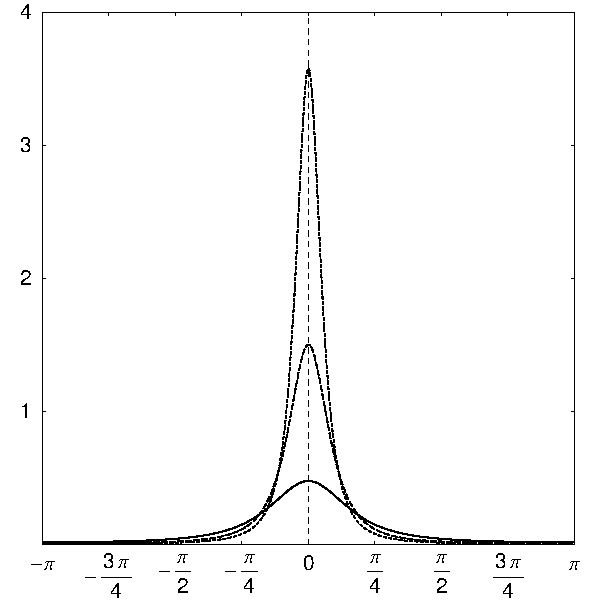
\includegraphics[width=0.45\textwidth]{images/poisson}}\hfill
  \subfigure[$\fun{S_{h}}{\cos\vartheta}$, $h=0.8,0.9,0.955$.]
  {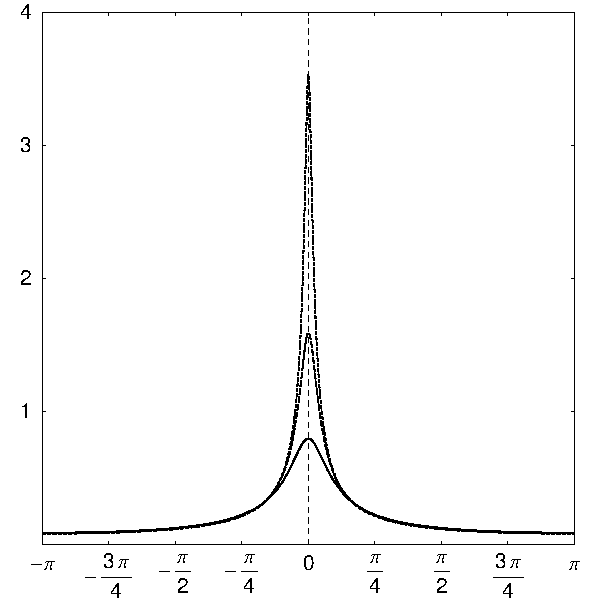
\includegraphics[width=0.45\textwidth]{images/singularity}}
  \caption{The kernels $\fun{Q_{h}}{\cos\vartheta}$ and $\fun{S_{h}}{\cos\vartheta}$
  for different values of $h$.}
  \label{Basics:Figure:PoissonSingularityKernel}
\end{figure}

For both kernels the Fourier-Legendre coefficients $\fun{K^{\wedge}}{k}$ are
explicitely known, such that we simply state the following lemma:

\begin{lemma}
  ${}^{}$\\[-2ex]
 \begin{enumerate}
   \item 
Using the Poisson kernel $K=Q_h$, cf. Definition \ref{def:poisson_sing} 1.,
in our summation algorithm yields a relative error of
     \begin{equation}
       \label{error:poisson}
       \frac{\left\|f - f_{M}\right\|_{\infty}}{\left\|\V{b}\right\|_1} \le
       \frac{h^{M+1}}{4\pi}
       \left(\frac{2M+1}{1-h}+\frac{2}{\left(1-h\right)^2}\right)\, .
     \end{equation}
     \item 
Using the singularity kernel $K=S_h$, cf. Definition \ref{def:poisson_sing}
2., in our summation algorithm yields a relative error of 
       \begin{equation}
         \label{error:singular}
         \frac{\left\|f - f_{M}\right\|_{\infty}}{\left\|\V{b}\right\|_1} \le
         \frac{h^{M+1}}{4\pi} \left(\frac{2M+1}{2\left(1-h\right)}+
           \frac{4M}{\left(1-h\right)^2}+
         \frac{4}{\left(1-h\right)^3}\right)\, .
       \end{equation}
 \end{enumerate}
\end{lemma}
\begin{proof}
The Fourier-Legendre coefficients are given by $\fun{Q_{h}^{\wedge}}{k}=h^k$ and
$\fun{S_{h}^{\wedge}}{k}=\frac{2}{2k+1}h^k$, respectively.
Using Lemma \ref{lemma:error} yields the assertions.
\end{proof}
  
Simply put, our scheme achieves (almost) accuracy $\epsilon$ for $M \ge \log\epsilon \,
/ \, \log h$.

\subsection{Locally supported kernel}
\begin{definition}
  Let $h \in \interv{(}{-1}{1}{)}$ and $\lambda \in \NZ$.
  The locally supported kernel
    $L_{h,\lambda}:\interv{[}{-1}{1}{]} \rightarrow \R$, considered in
    \cite{Sc97}, is defined by
    \[
    \fun{L_{h,\lambda}}{x} := 
    \left\{\begin{array}{l@{\quad \text{if} \quad}rcl} 
        0 & -1 &\le x \le& h, \\
        \frac{\lambda+1}{2\pi(1-h)^{\lambda+1}}\paren{x-h}^{\lambda} &  h & <  x \le& 1.
      \end{array}\right.
    \]
\end{definition}

Figure \ref{Basics:Figure:LKernel} shows the function $L_{h,\lambda}$ for
different values $h$ and $\lambda$.
\begin{figure}[tb]
  \centering
  \subfigure[$\lambda=1.0$]
  {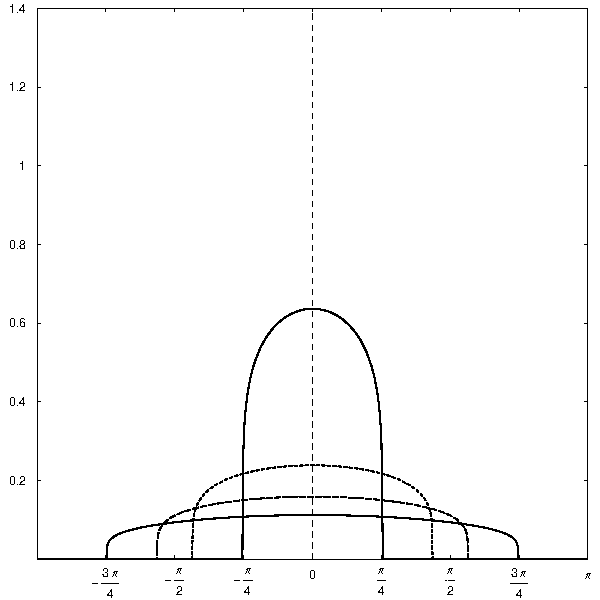
\includegraphics[width=0.45\textwidth]{images/locsup1}}\hfill
  \subfigure[$\lambda=2.0$]
  {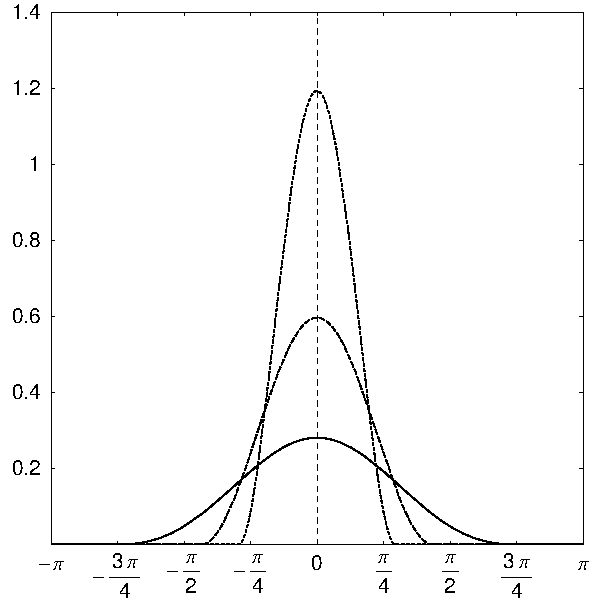
\includegraphics[width=0.45\textwidth]{images/locsup2}}
  \caption{The locally supported kernel $\fun{L_{h,\lambda}}{\cos\vtheta}$ 
  for $h = -0.7, 0.2, 0.7$ and different values of $\lambda$.}
  \label{Basics:Figure:LKernel}
\end{figure}
While the parameter $h$ again steers the localisation in spatial domain, the
parameter $\lambda$ correponds to the smoothness of $L_{h,\lambda}$ in the
endpoint of the support $h$.
We have the following lemma:

\begin{lemma}
  For the locally supported kernel $L_{h,\lambda}$ holds:
  \begin{enumerate}
  \item The Fourier-Legendre coefficients $\fun{L_{h,\lambda}^{\wedge}}{k}$ can be computed recursively by
    \[
    \fun{L_{h,\lambda}^{\wedge}}{k+1} = \frac{\paren{2k+1} h}{k+\lambda+2}
    \fun{L_{h,\lambda}^{\wedge}}{k}   - \frac{k-\lambda-1}{k+\lambda+2}
    \fun{L_{h,\lambda}^{\wedge}}{k-1}
    \]
    for $k\in \N$ where $\fun{L_{h,\lambda}^{\wedge}}{0} = 1$ and
    $\fun{L_{h,\lambda}^{\wedge}}{1} = \frac{\lambda + 1 + h}{\lambda+2}$.
  \item We obtain for $\lambda \in \NZ$ and $k>\lambda+1$ the decay rate
    \[
    \left|\fun{L_{h,\lambda}^{\wedge}}{k}\right| \le
    \frac{2\sqrt{2}}{\paren{2k+1}\sqrt{\pi}}
    \frac{\paren{\lambda+1}^2}{\paren{1-h}^{2\lambda+1}\sqrt[4]{1-|h|}}
    \frac{1}{\paren{k-\lambda}^{\lambda+\frac{1}{2}}}\,. 
    \]
  \item Thus, the relative error of our summation algorithm with this kernel
  $K=L_{h,\lambda}$ is bounded for $\lambda \in \N$ and $M>\lambda$ by
  \begin{equation}
    \label{error:Lh}
    \frac{\left\|f - f_{M}\right\|_{\infty}}{\left\|\V{b}\right\|_1} \le
    \frac{1}{\pi\sqrt{2\pi}}
    \frac{\paren{\lambda+1}^2}{\lambda-\frac{1}{2}}
    \frac{1}{\paren{1-h}^{2\lambda+1}\sqrt[4]{1-|h|}}
    \frac{1}{\paren{M-\lambda}^{\lambda-\frac{1}{2}}}\,.
  \end{equation}
  \end{enumerate}
\end{lemma}
\begin{proof}
  \begin{enumerate}
  \item We apply \eqref{three1} and \eqref{three2}.
  \item For $\lambda=0$, we have
    \begin{equation*}
      \left|\fun{L_{h,\lambda}^{\wedge}}{k}\right| 
      = \abs{2\pi \int_{h}^1 \frac{\lambda+1}{2\pi\paren{1-h}^{\lambda+1}} 
        \paren{x-h}^{\lambda} \fun{P_{k}}{x} \: \dx x} 
      \le \frac{\lambda+1}{(1-h)^{\lambda+1}}\abs{\int_{h}^1 \fun{P_{k}}{x} \: \dx x}.
    \end{equation*}
    Using \eqref{three2} and \eqref{leg_prop}, we obtain
    \begin{align*}
      \abs{\int_{h}^1 \fun{P_{k}}{x} \: \dx x}
      %& = \frac{1}{2k+1}
      %    \abs{\int_{h}^1 \fun{P_{k+1}'}{x} - \fun{P_{k-1}'}{x} \: \dx x}\\
      & = \frac{1}{2k+1}
          \abs{\fun{P_{k-1}}{h} - \fun{P_{k+1}}{h}}\\
      & \le \frac{1}{2k+1} \sqrt{\frac{2}{\pi \sin\arccos h}} \paren{\frac{1}{\sqrt{k-1}} + \frac{1}{\sqrt{k+1}}},
    \end{align*}
    and with $\sin\arccos h = \sqrt{1-h^2} \ge \sqrt{1-|h|}$ and
    $\frac{1}{\sqrt{k-1}} + \frac{1}{\sqrt{k+1}} \le
    \frac{2k+1}{k\sqrt{k}}$ finally
    \begin{equation}
      \label{SmallLambda}
      \left|\fun{L_{h,0}^{\wedge}}{k}\right| \le 
      \frac{\sqrt{2}}{\sqrt{\pi}}\frac{\lambda+1}{(1-h)^{\lambda+1}\sqrt[4]{1-|h|}}
      \frac{1}{k\sqrt{k}}.
    \end{equation}
%    \frac{1}{1-h}
%    \left|\int_{h}^{1} \fun{P_{k}}{x} \dx x\right| \le
%    \frac{\sqrt{2}}{\left(2k+1\right)\left(1-h\right)\sqrt{\pi}\sqrt[4]{1-h^2}}
%    \left(\frac{1}{\sqrt{k-1}}+\frac{1}{\sqrt{k+1}}\right)\,.
    Furthermore, for $\lambda \in \N$, we obtain by applying \eqref{three2} that
    \begin{equation*}
      \left|\fun{L_{h,\lambda}^{\wedge}}{k}\right| 
      %&\le&
      %\frac{\lambda+1}{\lambda\left(1-h\right)\left(2k+1\right)}
      %\left|\fun{L_{h,\lambda-1}^{\wedge}}{k-1}-
      %  \fun{L_{h,\lambda-1}^{\wedge}}{k+1}\right|\\ &\le&
      \le \frac{2}{2k+1} \frac{\lambda+1}{\lambda\left(1-h\right)}
      \max\limits_{|k-k'|\le 1}
      \left|\fun{L_{h,\lambda-1}^{\wedge}}{k'}\right|.
    \end{equation*}
    Iterate this argument and estimate $\frac{2}{2k'+1}\le
    \frac{1}{k-\lambda}$ yields
    \begin{align*}
      \left|\fun{L_{h,\lambda}^{\wedge}}{k}\right|
      & \le \frac{2}{2k+1} \frac{\lambda+1}{\paren{1-h}^{\lambda}}
        \frac{1}{\paren{k-\lambda}^{\lambda-1}} 
        \max_{|k-k'| \le \lambda} 
        \abs{\fun{L_{h,0}^{\wedge}}{k'}}.
    \end{align*}
    We finally use \eqref{SmallLambda} for $k'=k-\lambda$ to obtain the
    assertion.
  \item We combine 2. with Lemma \ref{lemma:error}. 
  \end{enumerate}
  \hfill
\end{proof}

Simply put, our scheme achieves accuracy of order $\epsilon$ for $M \ge
\lambda + (1-h)^{-2} {\epsilon}^{-1/\lambda}$.

\subsection{Spherical Gaussian kernel}
The spherical analog to the well-known \emph{Gaussian kernel} $\e^{-\sigma x^2}$ is the 
\emph{spherical Gaussian kernel}, see for example \cite{bahu01}.
\begin{definition}
  For $\sigma>0$, the spherical Gaussian kernel
  $G_{\sigma}:\interv{[}{-1}{1}{]} \rightarrow \R$ is given by
  \begin{equation}
    \label{GaussKernel}
    \nonumber
    \fun{G_{\sigma}}{x} := \e^{2\sigma x-2\sigma}\,.
  \end{equation}
\end{definition}

Figure \ref{Basics:Figure:GKernel} shows the spherical Gaussian kernel $G_{\sigma}$ for
different values $\sigma$.
\begin{figure}[tb]
  \centering
  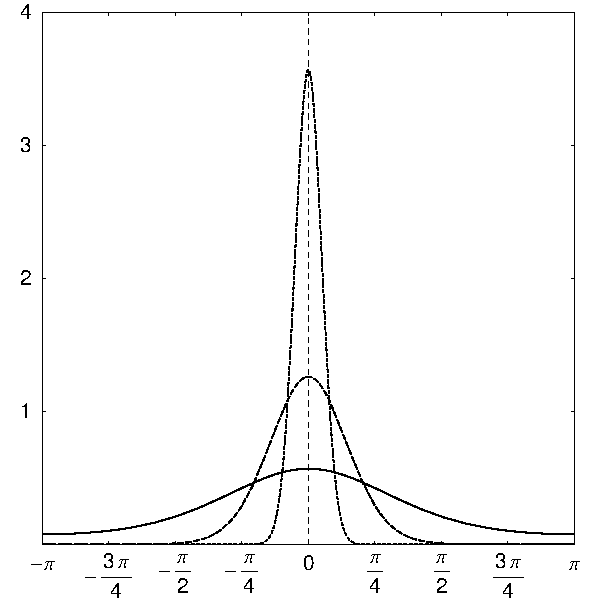
\includegraphics[width=0.7\textwidth]{images/gaussian}
  \caption{The $\text{L}^2$-normalized spherical Gaussian kernel 
  $\fun{\gamma}{\sigma} \fun{G_{\sigma}}{\cos\vtheta}$ with
  $\fun{\gamma}{\sigma} := \paren{\frac{2\sigma}{\pi}}^{1/2} \paren{1-\e^{-8\sigma}}^{-1/2}$ for $\sigma = 1,5,20$.}
  \label{Basics:Figure:GKernel}
\end{figure}

\begin{lemma}
For the spherical Gaussian $G_{\sigma}$ holds:
  \begin{enumerate}
  \item The Fourier-Legendre coefficients $\fun{G_{\sigma}^{\wedge}}{k}$
    are given by
    \begin{equation}
      \label{gaussian:explicit}
      \fun{G_{\sigma}^{\wedge}}{k} = 2 \sigma^{-\frac{1}{2}} \e^{-2\sigma}
      \pi^{\frac{3}{2}} I_{k+\frac{1}{2}}\left(2\sigma\right)
    \end{equation}
    where $I_{k+\frac{1}{2}}$ denotes the modified Bessel function of first
    kind, see \cite{abst}.
                                %Furthermore, $\fun{G_{\sigma}^{\wedge}}{k} \ge 0$.
  \item Thus, the relative error of our summation algorithm with the spherical Gaussian
    kernel $K=G_{\sigma}$ is bounded by
    \begin{equation}
      \label{error:G}
      \frac{\left\|f - f_{M}\right\|_{\infty}}{\left\|\V{b}\right\|_1} \le
      \frac{\sqrt{\pi\sigma}\left(\e^{\sigma}-1\right) \sigma^{M-\frac{1}{2}}}{\fun{\Gamma}{M
          +\frac{1}{2}}}.
    \end{equation} 
\end{enumerate}
\end{lemma}
\begin{proof}
  \begin{enumerate}
  \item The relation \eqref{three2} and integration by parts yields the
    difference equation
    \begin{equation}\label{eq:gauss_rec}
    {2\sigma}\fun{G_{\sigma}^{\wedge}}{k-1} - {2\sigma}\fun{G_{\sigma}^{\wedge}}{k+1} = 
    \left(2k+1\right)\fun{G_{\sigma}^{\wedge}}{k}
    \end{equation}
    for $k\in \N$ where $\fun{G_{\sigma}^{\wedge}}{0} = 4 \pi \sigma^{-1}
    \e^{-2\sigma} \sinh \sigma \cosh \sigma$ and
    $\fun{G_{\sigma}^{\wedge}}{1} = \pi \sigma^{-2} \e^{-2\sigma} (2 \sigma
    \cosh 2 \sigma + \sinh \sigma )$.
    The assertion follows e.g. by \cite{bahu01}.
  \item Using 1. and
  \begin{eqnarray*}
    \frac{2k+1}{4\pi} \abs{\fun{G_{\sigma}^{\wedge}}{k}}
    &=&
    \frac{\e^{-2\sigma}
    \left(k+\frac{1}{2}\right)\sigma^k}{\fun{\Gamma}{k+1}} \int_{-1}^{1}
    \e^{2\sigma x} \left(1-x^2\right)^k \dx x\\
    &\le&
    \frac{\left(k+\frac{1}{2}\right)\sigma^k}{\fun{\Gamma}{k+1}}
    \int_{-1}^{1} \left(1-x^2\right)^k \dx x\\
    &=&
    \frac{\sqrt{\pi}\sigma^k}{\fun{\Gamma}{k+\frac{1}{2}}}
  \end{eqnarray*}
  in conjunction with
  \begin{equation*}
    \sum_{k>M} \frac{\sqrt{\pi}\sigma^k}{\fun{\Gamma}{k+\frac{1}{2}}}\\
    =
    \frac{\sqrt{\pi\sigma}\e^{\sigma}}{\fun{\Gamma}{M+\frac{1}{2}}} 
    \int_{0}^{\sigma} t^{M-\frac{1}{2}} \e^{-t} \dx t\\
    \le
    \frac{\sqrt{\pi\sigma}\left(\e^{\sigma}-1\right)
    \sigma^{M-\frac{1}{2}}}{\fun{\Gamma}{M+\frac{1}{2}}}
  \end{equation*}
  yields the assertion.
\end{enumerate}
  \hfill
\end{proof}

Note that using the difference equation \eqref{eq:gauss_rec} in a forward
recursion is numerically unstable and we therefore use routines for
evaluating Bessel functions provided by
the \emph{GNU scientific library (GSL)} \cite{gsl} in the
precomputation of the Fourier-Legendre coefficients $\fun{G^{\wedge}}{k}$ 
by means of \eqref{gaussian:explicit}.

We conclude this section with the following corollary on the matrix norm
approximation.
\begin{corollary}
  \label{cor:rankapprox}
  Let $L \in \N$, a set of arbitrary source nodes $\mathcal{Y} =
  \pset{\V{\eta}_{l} \in \twosphere}{|}{l = 0,\ldots,L-1}$, and a set of
  arbitrary target nodes $\mathcal{X} := \pset{\V{\xi}_{l} \in
  \twosphere}{|}{l=0,\ldots,L-1}$ be given.
  Then, the proposed approximation $\V{Y_{\mathcal{X}}} \: \V{\hat W} \:
  \V{Y_{\mathcal{Y}}}^{\adj}$ to the matrix $\V{K}$, cf. Remark
  \ref{rem:rankM}, fulfils
  \begin{equation*}
    \left\| \V{K} - \V{Y_{\mathcal{X}}} \: \V{\hat W} \:
      \V{Y_{\mathcal{Y}}}^{\adj} \right\|_p
    \le L \: C_M
  \end{equation*}
  for $1\le p \le \infty$ where $C_M$ denotes the right hand sides in one of
  the inequalities \eqref{error:poisson}, \eqref{error:singular},
  \eqref{error:Lh}, or \eqref{error:G}. 
\end{corollary}
\begin{proof}
 Using Hoelders inequality, we obtain
 \[
 \left\| \V{K} - \V{Y_{\mathcal{X}}} \: \V{\hat W} \:
   \V{Y_{\mathcal{Y}}}^{\adj} \right\|_p
 = \max_{\V{b}\in \R^L} \frac{\left\|\V{f} -
     \V{f}_{M}\right\|_{p}}{\left\|\V{b}\right\|_p}
 \le \max_{\V{b}\in \R^L} L^{\frac{1}{p}} L^{1-\frac{1}{p}} \frac{\left\|\V{f}
     - \V{f}_{M}\right\|_{\infty}}{\left\|\V{b}\right\|_1}\,.
 \]
 The assertion follows by $\|\V{f} - \V{f}_{M}\|_{\infty} \le
  \|f-f_M\|_{\infty}$ and the estimates
  \eqref{error:poisson}, \eqref{error:singular}, \eqref{error:Lh}, or
  \eqref{error:G}.
\end{proof}

Using for example the Poisson kernel, we achieve an approximation of the square matrix
$\V{K}\in\R^{L \times L}$ up to an prescribed accuracy $\varepsilon$ by
choosing the truncation parameter $M\ge \log(\frac{\varepsilon}{L}) /\log h$.
Thus, for the Poisson kernel we have to increase the truncation parameter to
$M+\log\frac{1}{2} / \log h$ whenever we double the number of nodes to achieve
the same accuracy.

%%%%%%%%%%%%%%%%%%%%%%%%%%%%%%%%%%%%%%%%%%%%%%%%%%%%%%%%%%%%%%%%%%%%%%%%%%%%%%%
\section{Numerical results}
%%%%%%%%%%%%%%%%%%%%%%%%%%%%%%%%%%%%%%%%%%%%%%%%%%%%%%%%%%%%%%%%%%%%%%%%%%%%%%%

We present numerical examples in order to demonstrate the performance of
our approach. All algorithms were implemented in C and tested on an 
AMD Athlon\texttrademark XP 2700+ with 2GB main memory, SuSE-Linux 
(kernel 2.4.20-4GB-athlon, gcc 3.3) using double precision arithmetic. 
Moreover, we have used the libraries FFTW 3.0.1 \cite{fftw}, NFFT 2
\cite{kupo02C} and a custom NFSFT library which will be part of the next 
major release of the NFFT library. Throughout our experiments we have 
applied the NFFT package \cite{kupo02C} with precomputed Kaiser--Bessel 
functions and an oversampling factor $\rho=2$.

In our tests we have always chosen uniformely distributed pseudo-random 
source and target nodes 
$\paren{\vartheta,\varphi} \in [0,\pi] \times [-\pi,\pi)$ and 
coefficients $b_l$ from $\left[-\frac{1}{2},\frac{1}{2}\right]$.

We have considered the following kernels:

\begin{itemize}
  \item Poisson kernel $Q_{h}$,
  \item singularity kernel $S_{h}$,
  \item locally supported kernel $L_{h,\lambda}$,
  \item Gaussian kernel $G_{\sigma}$.
\end{itemize}

First, we examine the systematic error due to our approximation
\eqref{Applications:TruncatedSeries} and the use of the approximative NFSFT
algorithms. Figure \ref{fig:error} shows the error
\[
E_{\infty}:=
\frac{\left\|\V{f}-\V{f}_M\right\|_{\infty}}{\left\|\V{b}\right\|_{1}}
\quad \approx \quad \frac{\left\|f-f_M\right\|_{\infty}}{\left\|\V{b}\right\|_{1}}
\]
for the mentioned kernels as a function of the cutoff degree $M$.
These results confirm the error estimates \eqref{error:poisson},
\eqref{error:singular}, \eqref{error:Lh}, and \eqref{error:G}.

\begin{figure}[tb]
  \centering
  \subfigure[The Poisson kernel $Q_{h}$ for $h = 0.8$.]
  {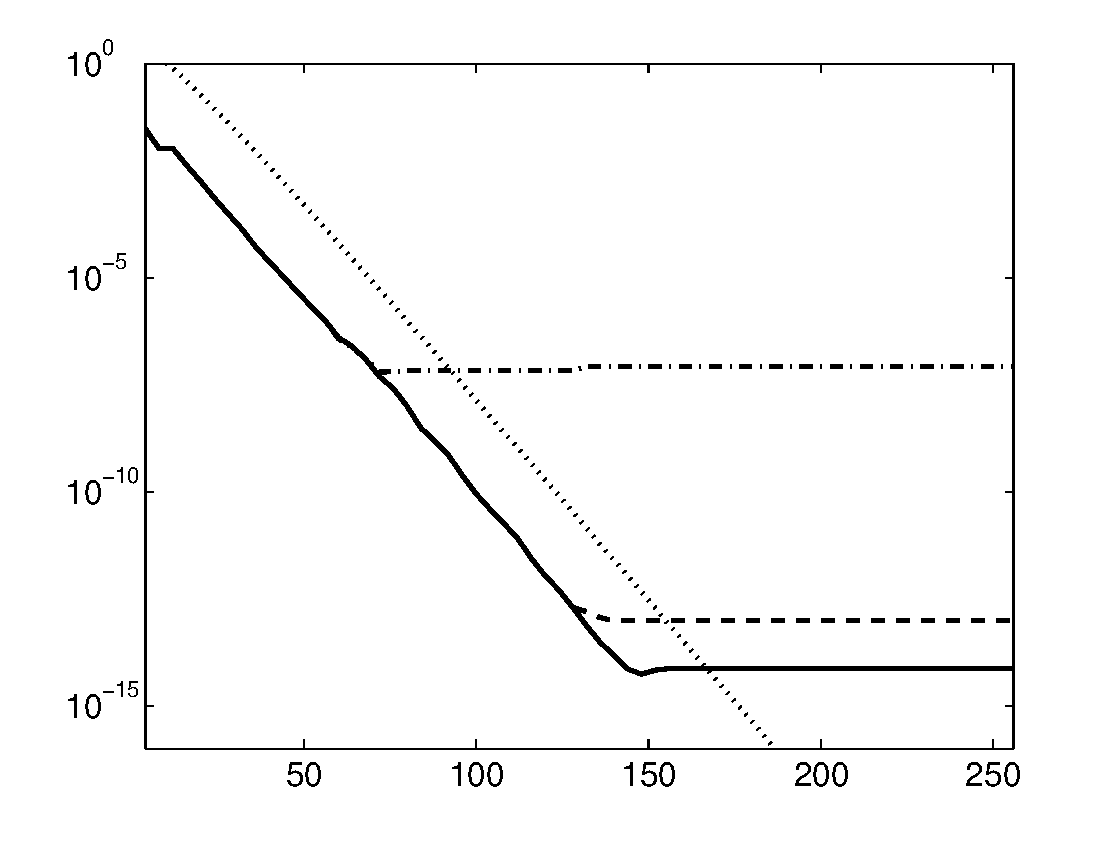
\includegraphics[width=0.45\textwidth]{images/poisson_test}}\hfill
  \subfigure[The Singularity kernel $S_{h}$ for $h = 0.8$.]
  {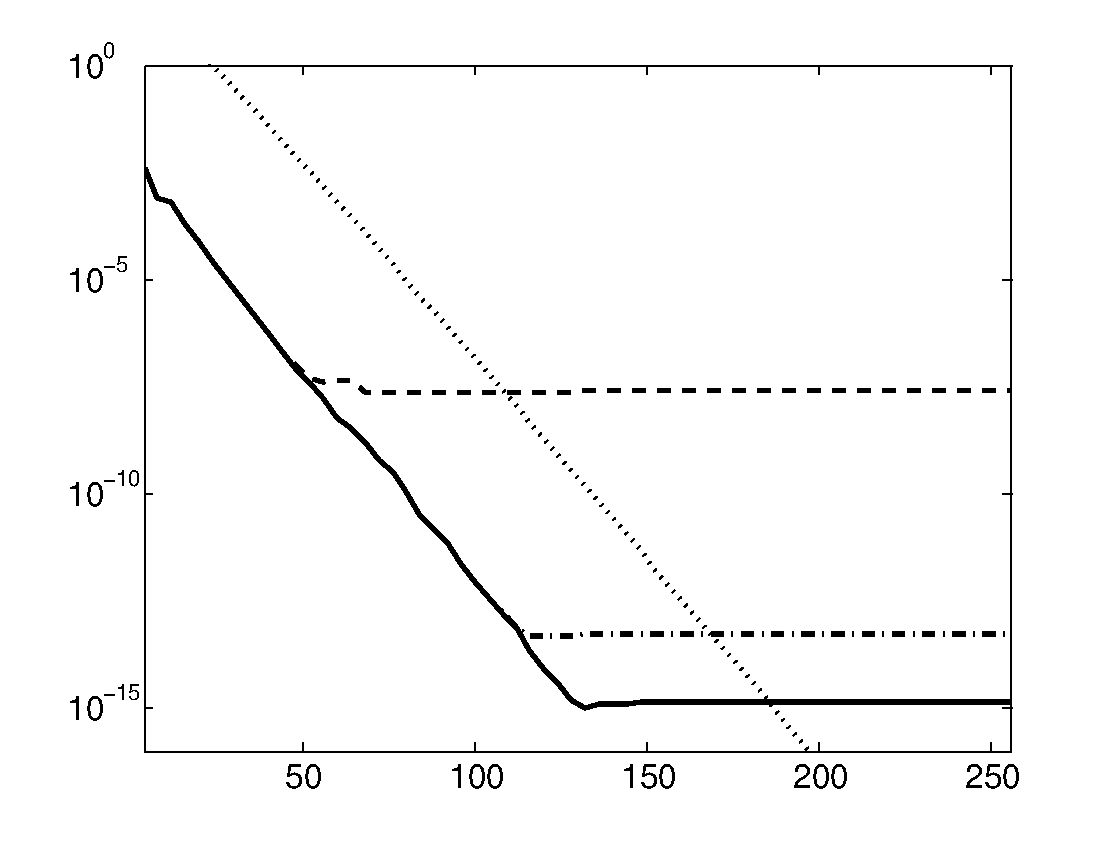
\includegraphics[width=0.45\textwidth]{images/singularity_test}}\\
  \subfigure[The locally supported kernel $L_{h,\lambda}$ for $h=0.3$ and $\lambda = 7$.]
  {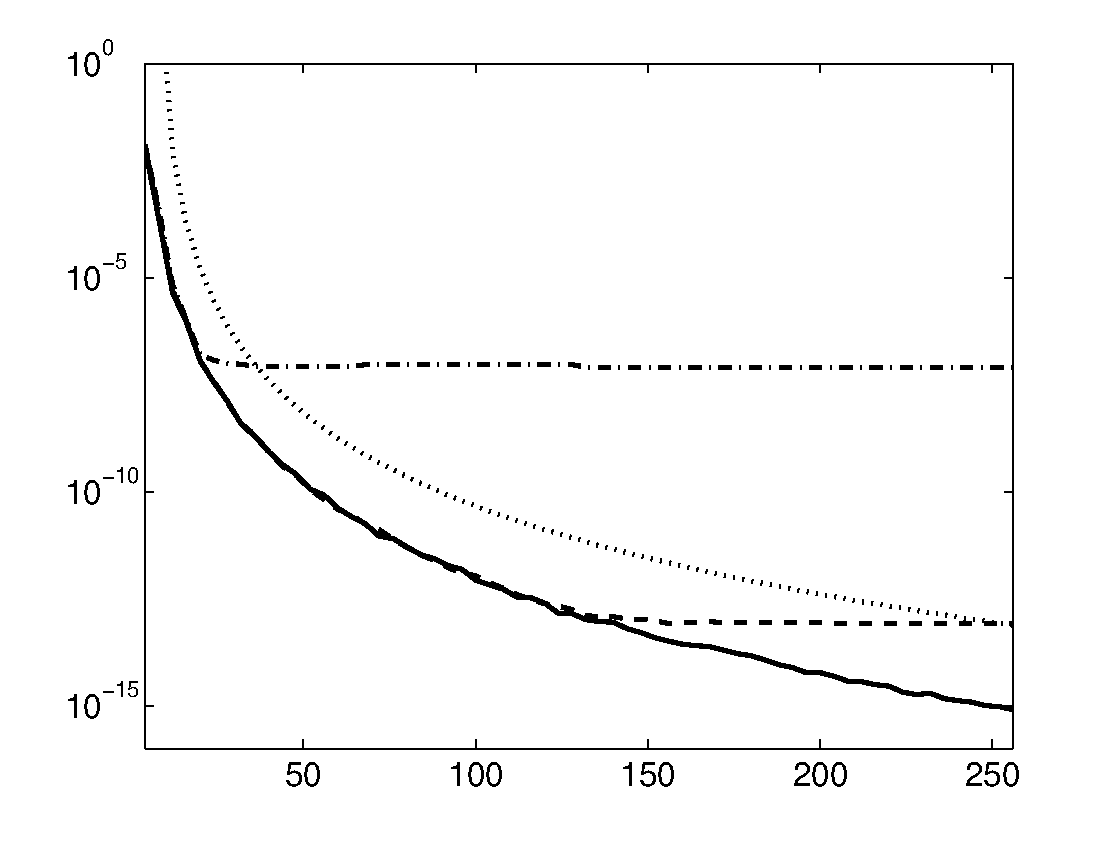
\includegraphics[width=0.45\textwidth]{images/locsupp_test}}\hfill
  \subfigure[The Gaussian kernel $G_{\sigma}$ for $\sigma=100$.]
  {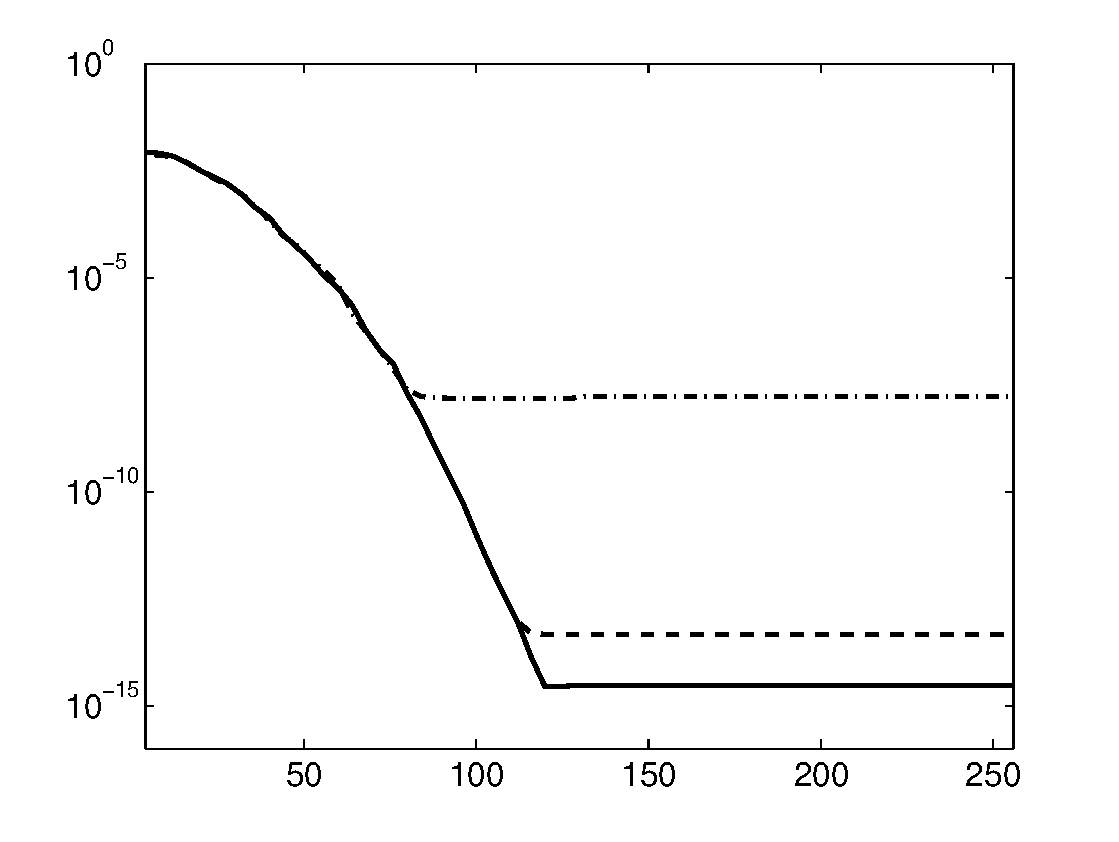
\includegraphics[width=0.45\textwidth]{images/gaussian_test}}
  \caption{The error $E_{\infty}$ for $M = 4,8,\ldots,256$ and $L = D = 1000$: 
  Fast summation with NDSFT (solid), fast summation with NFSFT and 
  NFFT cutoff parameter $m = 3$ (dash-dot), fast summation with NFSFT and NFFT cutoff 
  parameter $m = 6$ (dashed), error estimate for 
  $E_{\infty}$ (dotted).}
  \label{fig:error}
\end{figure}

\begin{figure}[tb]
  \centering
  \subfigure[The Poisson kernel $Q_{h}$ for $h = 0.8$: Fast summation with 
  NFSFT/NDSFT and thresholds $10^6$ (solid), $10^9$ (dashed), $10^9$ (dash-dot). 
  The threshold steers the accuracy of the FLFT transformation.]
  {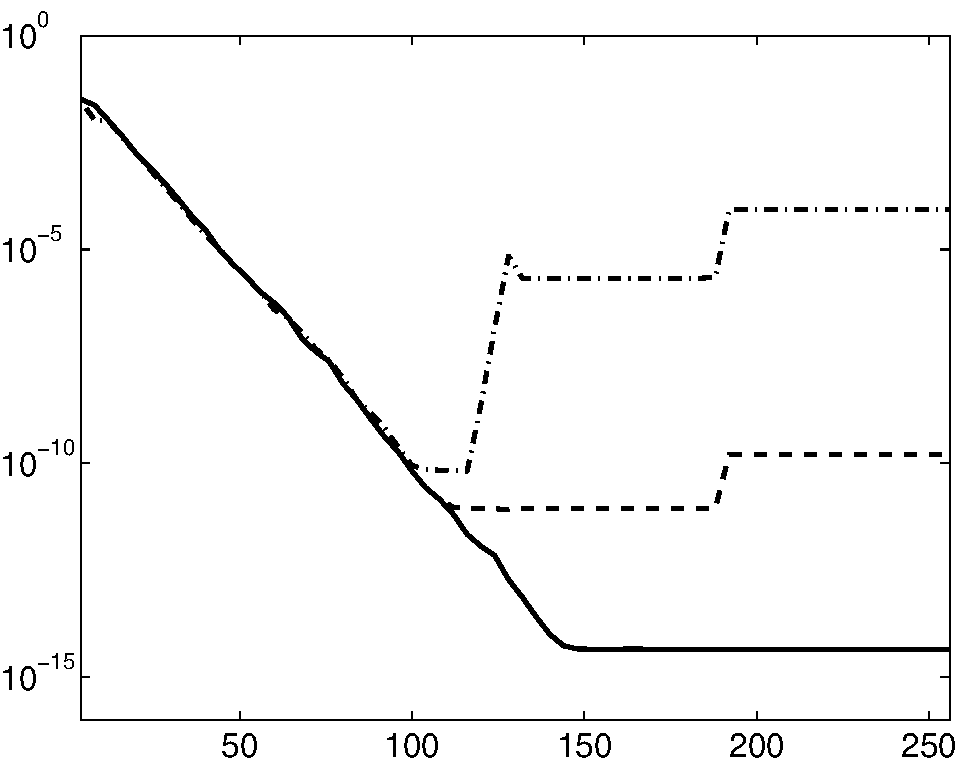
\includegraphics[width=0.45\textwidth]{images/threshold_test}}\hfill
%  \subfigure[The locally supported kernel $L_{h,\lambda}$ for $\lambda = 7$, and $h=0.3$ (solid),
%  and $h=0.7$ (dashed). The error estimate (dotted) for $E_{\infty}$ was fitted 
%  using $C_{\lambda} = 100$.]
%  {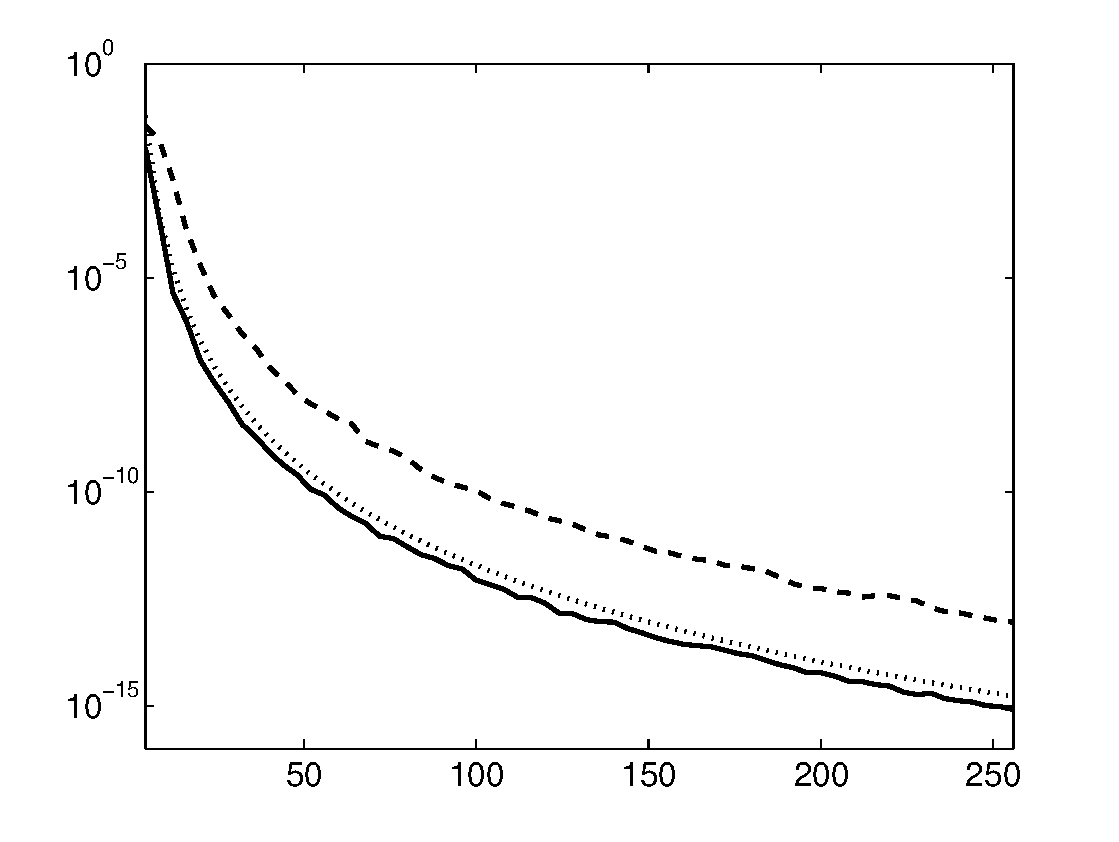
\includegraphics[width=0.45\textwidth]{images/locsup_h_test}}
  \caption{The error $E_{\infty}$ for $M = 4,8,\ldots,256$ and $L = D = 1000$.}
  \label{Figure:PoissonTest}
\end{figure}

We now compare the computation time of the straightforward summation, the
straightforward summation with precomputed matrix $\V{K}$, the fast summation
algorithm with NDSFT, and the fast summation algorithm with NFSFT for
increasing $D=L$ and fixed cutoff degree $M=128$. 
The CPU time required by the four algorithms is shown in Table
\ref{tab:TimeSpace}. 
As expected, the fast NDSFT and NFSFT summation algorithms outperform the 
straightforward algorithms, but with the NFSFT--version considerably faster.

\begin{table}[ht!]
  \begin{center}
    \begin{tabular}{r|r|r|r|r|r}
         $L = D$ &      direct alg.   &     w/precomp.     &      FS, NDSFT &      FS, NFSFT & error $E_{\infty}$\\\hline\\[-2.0ex]
           $2^6$ & \verb#1.0E-05#     & \verb#8.0E-05#     & \verb#1.1E-01# & \verb#6.2E-01# & \verb#7.7E-14# \\
           $2^7$ & \verb#6.0E-05#     & \verb#3.8E-04#     & \verb#2.2E-01# & \verb#6.2E-01# & \verb#6.5E-14# \\
           $2^8$ & \verb#2.5E-04#     & \verb#1.4E-03#     & \verb#4.5E-01# & \verb#6.2E-01# & \verb#4.1E-14# \\
           $2^9$ & \verb#1.0E-03#     & \verb#5.3E-03#     & \verb#8.9E-01# & \verb#6.3E-01# & \verb#2.8E-14# \\
        $2^{10}$ & \verb#4.0E-02#     & \verb#2.1E-02#     & \verb#1.8E+00# & \verb#6.5E-01# & \verb#3.6E-14# \\
        $2^{11}$ & \verb#1.6E+00#     & \verb#8.3E-02#     & \verb#3.6E+00# & \verb#6.6E-01# & \verb#1.8E-14# \\
        $2^{12}$ & \verb#6.4E+00#     & \verb#3.5E-01#     & \verb#7.1E+00# & \verb#7.2E-01# & \verb#1.3E-14# \\
        $2^{13}$ & \verb#2.6E+01#     & \verb#1.4E+00#     & \verb#1.4E+01# & \verb#8.2E-01# & \verb#6.7E-15# \\
        $2^{14}$ & \verb#1.0E+02#     & $^*$\verb#5.6E+00# & \verb#2.8E+01# & \verb#1.0E+00# & \verb#5.5E-15# \\
        $2^{15}$ & \verb#4.1E+02#     & $^*$\verb#2.2E+01# & \verb#5.7E+01# & \verb#1.5E+00# & \verb#4.0E-15# \\
        $2^{16}$ & \verb#1.6E+03#     & $^*$\verb#8.9E+01# & \verb#1.1E+02# & \verb#2.3E+00# & \verb#2.9E-15# \\
        $2^{17}$ & \verb#6.6E+03#     & $^*$\verb#3.6E+02# & \verb#2.3E+02# & \verb#4.0E+00# & \verb#2.4E-15# \\
        $2^{18}$ & \verb#2.6E+04#     & $^*$\verb#1.4E+03# & \verb#4.6E+02# & \verb#7.5E+00# & \verb#1.9E-15# \\
        $2^{19}$ & $^*$\verb#1.0E+05# & $^*$\verb#5.7E+03# & \verb#9.1E+02# & \verb#1.4E+01# & \verb#-# \\
        $2^{20}$ & $^*$\verb#4.2E+05# & $^*$\verb#2.3E+04# & \verb#1.8E+03# & \verb#2.8E+01# & \verb#-# \\
        $2^{21}$ & $^*$\verb#1.7E+06# & $^*$\verb#9.1E+04# & \verb#3.6E+03# & \verb#5.5E+01# & \verb#-# \\
    \end{tabular}

  \end{center}
  \caption{CPU-Time and error $E_{\infty}$ for the fast summation algorithm with cutoff degree $M = 128$.
    Note that we used accumulated measurements in case of small times. Values 
    marked with $^{*}$ are estimates owing to CPU-time and memory limitations.}
  \label{tab:TimeSpace}
\end{table}

As an example for the result provided by Corollary \ref{cor:rankapprox}, we 
finally consider the Poisson kernel $Q_{h}$ for 
$h = 0.1$ and $h=0.5$, $L=D=400$ arbitrary source and target nodes $\V{\eta}_{l}$ and $\V{\xi}_{d}$,
and our particular rank $(M+1)^2$ approximation 
$\V{Y_{\mathcal{X}}} \: \V{\hat W} \: \V{Y_{\mathcal{Y}}}^{\adj}$ to the matrix $\V{K} \in \R^{L \times L}$ 
for cutoff degrees $M=0,\ldots,19$. Note that for $M=19$ we 
have $(M+1)^2 = 400 = L = D$ and therefore $\V{Y_{\mathcal{X}}}, \V{\hat W}, 
\V{Y_{\mathcal{Y}}}^{\adj} \in \C^{L \times L}$ which renders our approximation a full-rank 
approximation. We compare the performance of our approach $\V{Y_{\mathcal{X}}} \: \V{\hat W} \: 
\V{Y_{\mathcal{Y}}}^{\adj}$ and the corresponding error estimate from Corollery \ref{cor:rankapprox}
with the truncated-SVD rank $l$ approximation $\V{S}_{l}$ for $l = 1,\ldots,L$
measured in the spectral norm $\left\|\cdot\right\|_{2}$. The results are shown in Figure \ref{fig:rankapprox}. 

\begin{figure}[tb]
  \centering
  \subfigure[$h=0.1$]
  {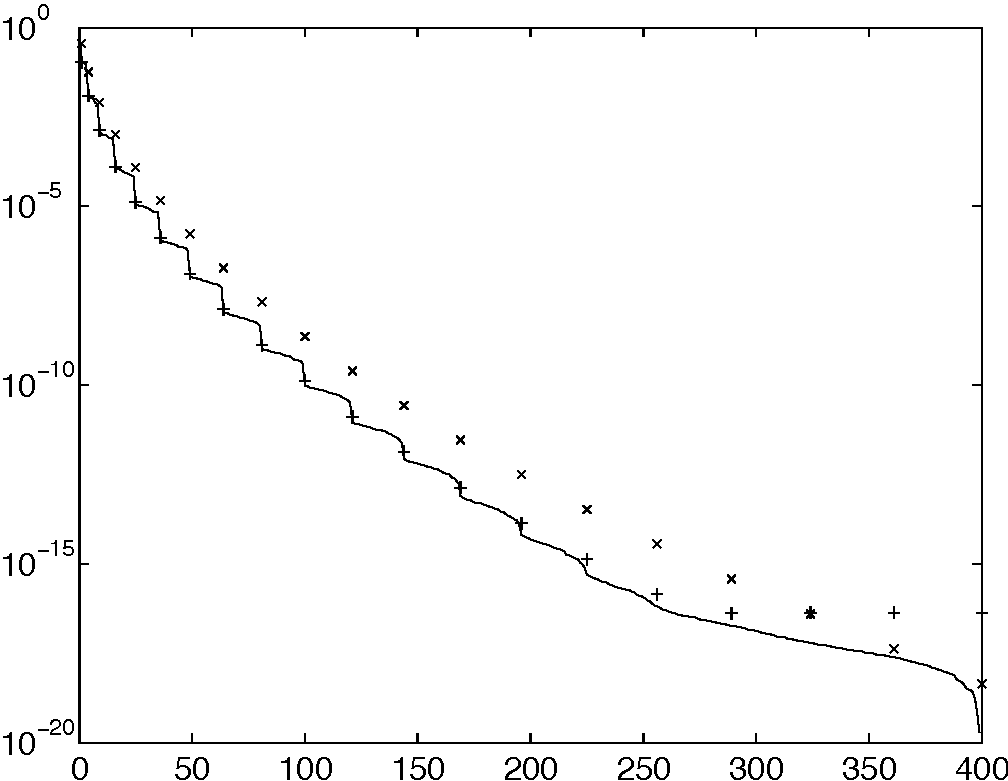
\includegraphics[width=0.45\textwidth]{images/poisson_h_0_1}}\hfill
  \subfigure[$h=0.5$]
  {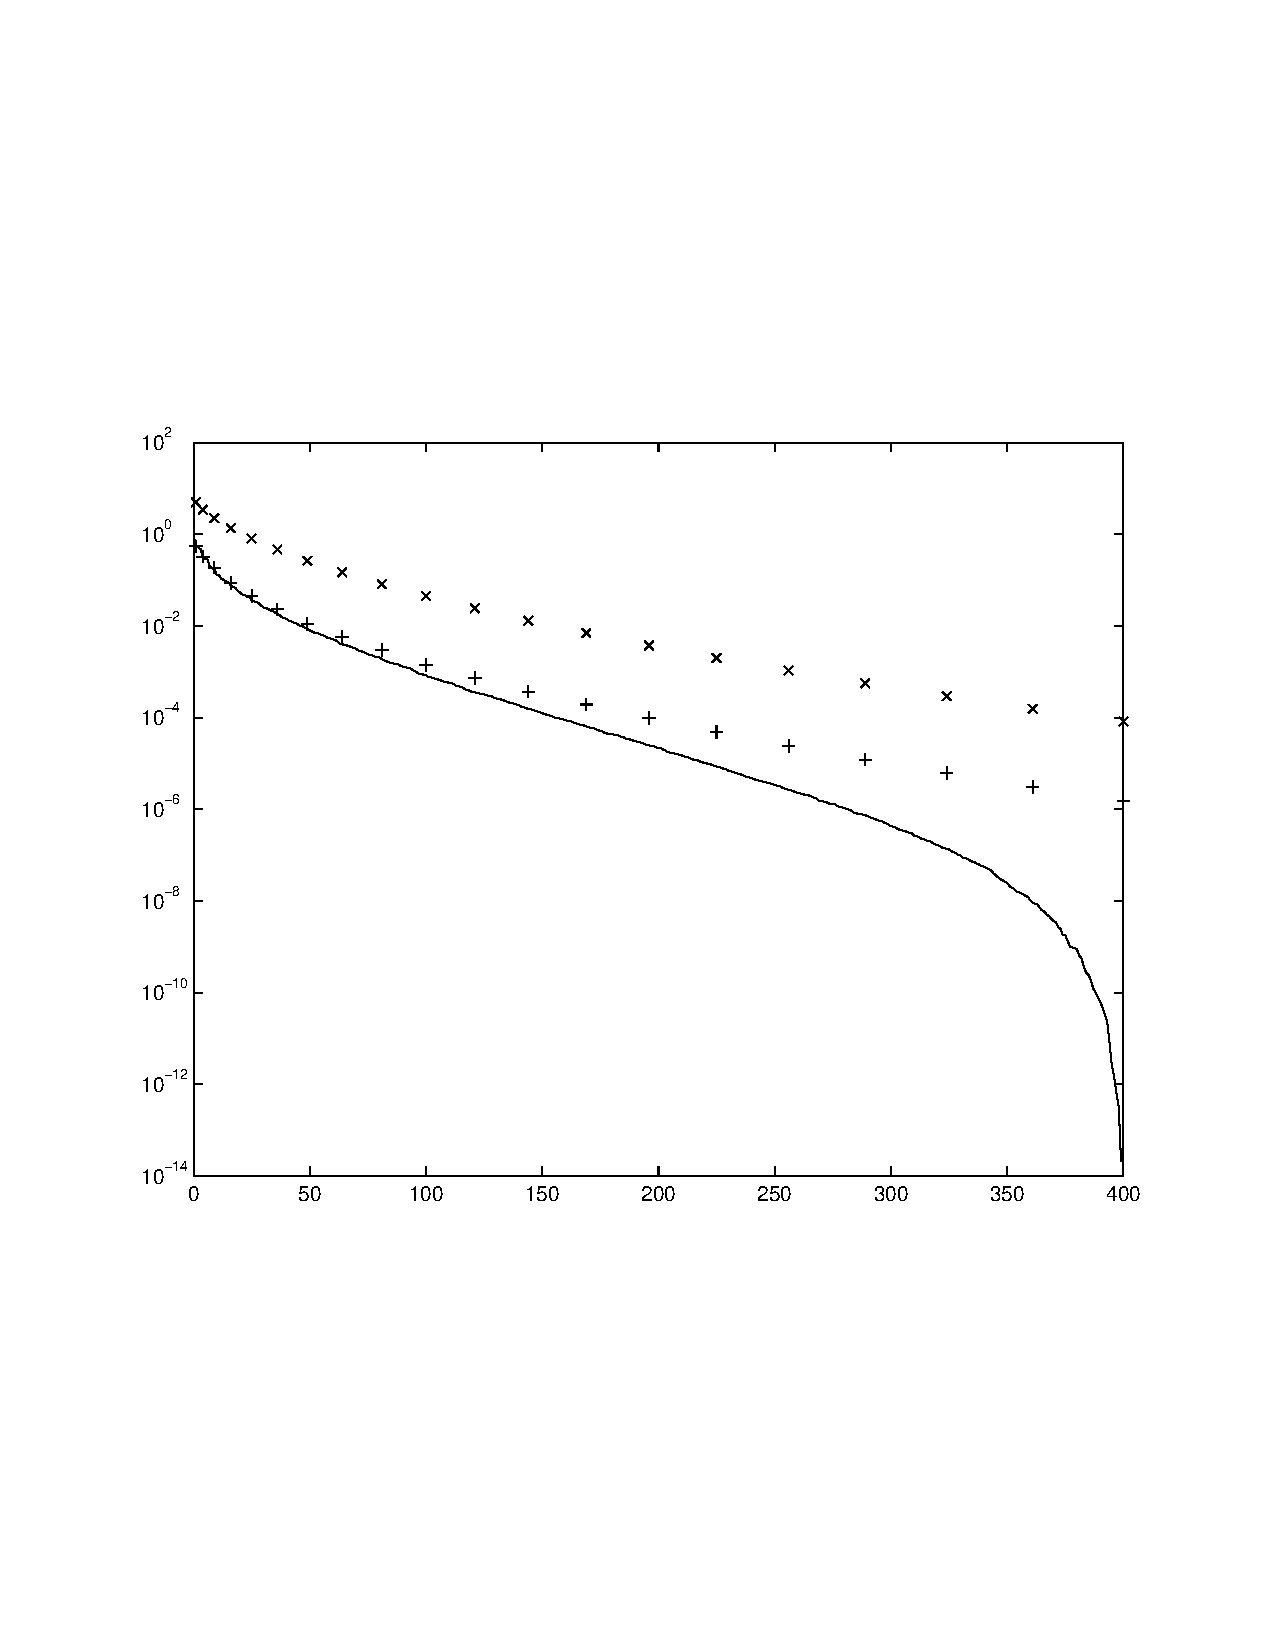
\includegraphics[width=0.45\textwidth]{images/poisson_h_0_5}}\\
  \caption{Comparison of our approximation $\V{Y_{\mathcal{X}}} \: \V{\hat W} \: 
  \V{Y_{\mathcal{Y}}}^{\adj}$ to the matrix $\V{K}$ with the truncated-SVD approximation
  for the Poisson kernel $Q_{h}$ with $h=0.1$ (left) and $h=0.5$ (right), 
  and $L = D = 400$ arbitrary source and target nodes. 
  We compare 
  $\|\V{K} - \V{Y_{\mathcal{X}}} \: \V{\hat W} \: \V{Y_{\mathcal{Y}}}^{\adj}\|_{2}$ 
  ($+$) and the error estimate $L \: C_{M}$ ($\times$) from Corollary \ref{cor:rankapprox} 
  for cutoff degree $M=0,\ldots,19$ with 
  $\left\|\V{K} - \V{S}_{l}\right\|_{2}$ (solid) for 
  the truncated-SVD rank $l$ approximation $\V{S}_{l}$ for $l=1,\ldots,L$.
  }
  \label{fig:rankapprox}
\end{figure}


%--------------------------------------------------------------------------
\section{Conclusions}
%--------------------------------------------------------------------------

We have presented a fast algorithm for the computation of sums of type
\eqref{Applications:KernelSum} in ${\cal O} (D + L)$ arithmetic operations.
For a range of zonal functions, we established error estimates 
concerning the dependence of the computational speed on the desired accuracy 
and the function's parameters. The numerical results confirm the theoretical 
expectations.
The software for this algorithm including all described tests can be
obtained from the authors.

%-----------------------------------------------------------------------------
\bibliographystyle{abbrv}
\bibliography{../references}
\end{document}
